\begin{figure*}%
	\centering%
	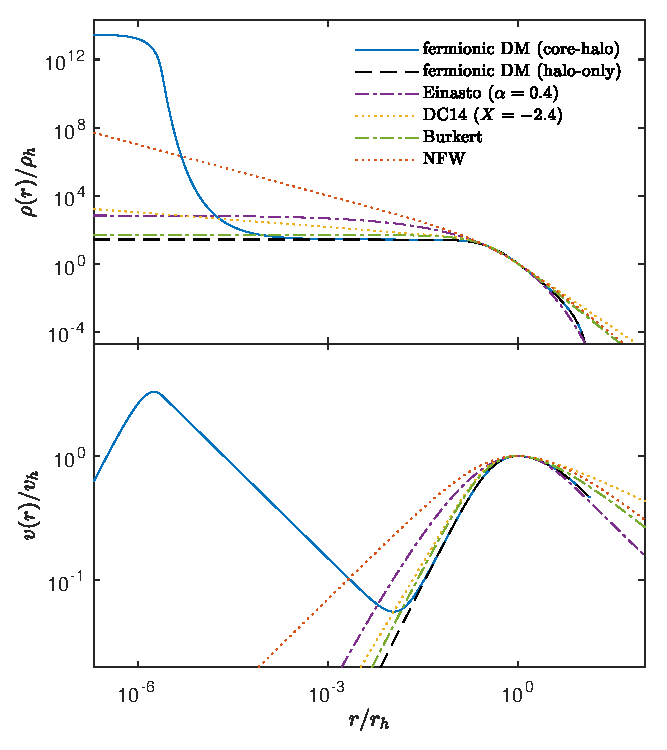
\includegraphics[width=\hsize]{\ROOTPATH/fig.pdf}%
	\caption{Total rotation curves and their composition, shown for UGC05986 (left), DDO161 (center) and NGC6015 (right). The thick lines are the best-fits of three competing DM models: Fermionic (blue), DC14 (yellow) and NFW (red). For clarity we have excluded Einasto.}%
	\label{fig:benchmark:total-rotation-curves}%
\end{figure*}